\documentclass[12pt, titlepage]{article}

\usepackage{booktabs}
\usepackage{tabularx}
\usepackage{hyperref}
\usepackage{graphicx}
\usepackage{float}
\hypersetup{
    colorlinks,
    citecolor=black,
    filecolor=black,
    linkcolor=red,
    urlcolor=blue
}
\usepackage[round]{natbib}

\usepackage{ulem}
\usepackage{xcolor}
\usepackage{color,array}


\title{SE 3XA3: Software Requirements Specification\\Spaceshooter Remix}

\author{Team \#4, IRS Development
		\\ Ibrahim Malik maliki2
		\\ Ryan Schnekenburger schneker
		\\ Saad Khan khans126
}

\date{\today}

\begin{document}

\maketitle

\pagenumbering{roman}
\tableofcontents
\listoftables
\listoffigures

\newpage

\begin{table}[hp]
\caption{Revision History} \label{TblRevisionHistory}
\begin{tabularx}{\textwidth}{llX}
\toprule {\bf Date} & {\bf Version} & {\bf Notes}\\
\midrule
October 3, 2018 & Rev0 & Authored by Ibrahim, Saad, Ryan\\
November 25, 2018 & Rev1 & Updated document and added the changes recommended by TA including rewriting subsection 2.1 and the requirements sections.\\
\bottomrule
\end{tabularx}
\end{table}

\noindent This document describes the requirements for Spaceshooter Remix written by IRS Development.

\newpage

\pagenumbering{arabic}

\section{Project Drivers}

\subsection{The Purpose of the Project}

The purpose of this project is to reinvent the popular retro game Spaceshooter. We aim to do this for the people who enjoy playing video games in their free time and want to get the feeling that they had when they were younger playing on their handheld consoles. This game was originally created for an early 70's era handheld console, however, these handheld game consoles are not very durable and not many are around today so it is difficult for people to play Spaceshooter. People also do not want to have to carry around a device to only play Spaceshooters everywhere they go, they seek the convenience in having the game on something that they usually carry around with them, their laptop. The final game should give people the retro feel that they crave, only it will be using Python.  

\subsection{The Stakeholders}
 

\subsubsection{The Client}

The client who we are creating this project for is the professor and TAs of the course who have instructed us to create an open-ended program that will be created in four months. They have greenlit us to create Space Shooter and will be the party interested in the final product to go out to the general public.

\subsubsection{The Customers}

The customers are people of the general public who will play our game. We seek their validation that all of our requirements have been properly executed in a way that keeps their attention on our game and has a positive experience. Specifically, the people of the general product who will consume our game are those who have a computer that runs either \textcolor{red}{Mac OSX, Windows or Linux machines}. The people who will consume our game will also be running the latest version of \textcolor{red}{Python} on their computer. 

\subsubsection{Other Stakeholders}

Future Developers
We aim to carefully document this project so that it could be picked up in the future by developers who would like to add to our idea. We must follow strict naming conventions and keep the document consistent to those who wish to add on to what we have updated.

\newpage

\subsection{Mandated Constraints}

\subsubsection{Solution Constraints}

Description: The product shall use the newest version of Python\\
Rationale: The product is originally coded on Python 2.6 and we only wish to update it not switch the language\\
Fit Criterion: The product shall run without any errors on Python 3.7 and the tests will all pass \\ \\
Description: The product shall run on all Windows, \textcolor{red}{Mac OSX}, and Linux machines\\
Rationale: These are the most popular operating systems and it would be impractical and unnecessary to create it for more obscure operating systems.\\
Fit Criterion: The product shall pass all tests when run on Windows, Mac OSX, and Linux machines.

\subsubsection{Partner or Collaborative Applications}

This product does not have any partner or collaborative applications. This product does, however, use some open source audio and graphics files.

\subsubsection{Off-the-shelf Software}

The product requires two types of off-the-shelf software:
\begin{itemize}
\item The newest version of \textcolor{red}{Python} (Available at https://www.python.org/downloads/)
\item A computer that runs Mac OSX, Windows, or Linux operating systems
\end{itemize}

\subsubsection{Anticipated Workplace Environment}

The game should be played when the computer keyboard or laptop is at an arm's length away. The computer should be on a flat surface. The product also does not need an Internet connection so you could play this game anywhere. 

\subsubsection{Schedule Constraints}

The client's deadline to complete this project is \sout{at the beginning of December} \textcolor{red}{December 5, 2018. The presentation of the final product has to be completed by November 26, 2018.} However, we could continue to update the game for as long as we want.

\subsubsection{Budget Constraints}

There are no budget constraints. We were provided with the source code needed to re-create the project and as such no budget is necessary.

\newpage

\subsection{Naming Conventions and Terminology}

\begin{table}[H]
\caption{Name Convensions table and Terminology}
\begin{tabular}{ |p{5cm}|p{8cm}|}
\hline
 Acronyms/Abbreviations &  Meaning \\ \hline
 OS &  Operating System  \\ \hline
 product & The game that we are creating   \\ \hline
 program & The code that our game uses to function   \\ \hline
 ex. & example \\ \hline
 etc. & et cetera \\ \hline
 client & Who we are creating the game for \\ \hline
 customer & Who will be consuming our game \\ \hline
\textcolor{red}{sprite} & \textcolor{red}{The spaceship displayed on the screen representing the user's character}  \\ \hline
 Git repo& \textcolor{red}{Gitlab repository} \\ \hline
\textcolor{red}{player} & \textcolor{red}{The human playing the game or using the software}\\ \hline
\textcolor{red}{user} & \textcolor{red}{The human playing the game or using the software}\\ \hline
 IDLE & The integrated development environment for \textcolor{red}{Python} \\ \hline
 repo & The repository where our product will be stored \\ \hline
\end{tabular}
\end{table}


\newpage

\subsection{Relevant Facts and Assumptions}

\subsubsection{Relevant Facts}
The game was originally 600 lines of code. The game is licensed under MIT. The code for the original game is located at https://github.com/tasdikrahman/spaceShooter.

\subsubsection{Assumptions}

The assumptions are that the software that will be used to develop this project will be free and available to us. The object and sound files will be free for public consumption. 
\newline
\\Other assumptions include the target user's characteristics which include:
\begin{itemize}
\item Physical abilities $\Rightarrow$ They are able to operate a keyboard and mouse/track-pad
\item Technical abilities $\Rightarrow$ Competent with downloading and running \textcolor{red}{Python} programs
\item \sout{Attitude toward job $\Rightarrow$ Indifferent}
\item \sout{Attitude toward technology $\Rightarrow$ They are positive towards technology}
\item Education $\Rightarrow$ Completed elementary school
\item Linguistic skills $\Rightarrow$ They are competent in English
\item \sout{Age $\Rightarrow$ In the age of majority}
\item \sout{Gender $\Rightarrow$ Male or Female it is unrelated}
\end{itemize}

\newpage

\section{Functional Requirements}

\subsection{The Scope of the Project and the Product}

\subsubsection{The Scope of the Project}

\textcolor{red}{The current Spaceshooter game that uses user inputs from a keyboard and displays a player sprite on the computer screen. The actions of the user result in the movement of the spaceship and hitting the spacebar button will fire bullets to destroy the oncoming asteroids. Sound is also released from the speakers. Our reimplemented game shall change some of these functions by adding an increased level of difficulty and switch the input controls for shooting from spacebar to a mouse. Movement of the player sprite will be controlled by the `A' and `D' keys on the keyboard.}
\newline
\\Below are the set of deliverables and deadlines for this project.
\newline
\\Deliverables:
\begin{itemize}
    \item Requirements Documentation
    \item Functioning software
\end{itemize}

\noindent Deadlines:
\begin{itemize}
    \item Proof of Concept Demonstration October 15
    \item Test Plan (Revision 0) October 26
    \item Design and Document (Revision 0) November 9
    \item Revision 0 Demonstration November 12
    \item Final Demonstration (Revision 1) November 26
    \item Final Documentation (Revision 1) November 26
    \item Final Documentation (Revision 1) December 5
\end{itemize}

\subsubsection{Context of the Work}
\begin{figure}[H]
\centering
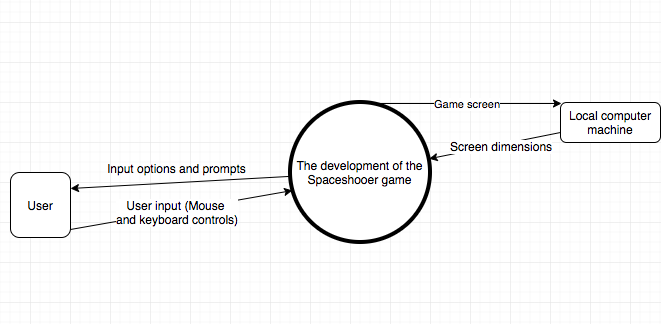
\includegraphics[scale=0.5]{CONTEXTDIAGRAM}
\caption{\textcolor{red}{The Context of the Work}}
\end{figure}

 
\subsubsection{Work Partitioning}
 

\begin{table}[H]
\caption{Work Partitioning}
{
\color{red} \begin{tabular}{ |p{4cm}|p{4cm}|p{4cm}| }
\hline 
Event Name  & Input and Output  & Summary \\ \hline
        1 . User uses keyboard and mouse controls &  Keyboard and mouse  &  User's spaceship will move and shoot based off their selections  \\ \hline
        2 . User starts the game        &  Keyboard    &  The game begins and the score starts to record    \\ \hline 
        3 .  User closes the game         &   Keyboard  &  The game exits to desktop and shuts down    \\ \hline
        4 .  User runs game from executable          &   Mouse   &    This initiates the game in Python   \\ \hline
\end{tabular}
}

\end{table}


\subsubsection{Use Case}
The main use case for this project if for entertainment purposes. The game is being created to provide enjoyment out of creating high scores and gameplay.

\begin{figure}[H]
\centering
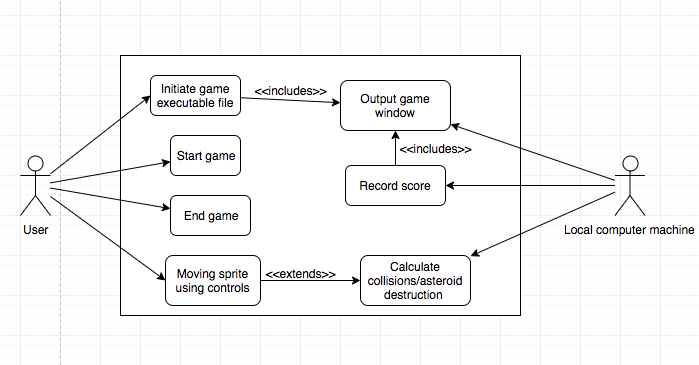
\includegraphics[scale=0.5]{USECASE}
\caption{\textcolor{red}{Use Case Diagram for Spaceshooter }}
\end{figure}

\subsection{Functional Requirements}

\subsubsection{Functional Requirements}
Requirement number: F1
\\When the game is executed in \textcolor{red}{Python}, a new window shall be opened.
\\Fit Criterion or Test Case: \sout{Is a new window opened after the program is executed?}
\textcolor{red}{A new window will open on the computer screen after the program is executed.}
\bigskip

\noindent Requirement number: F2
\\The game shall open a main menu once executed in \textcolor{red}{Python, Linux, Mac OSX or Windows.}
\\Fit Criterion or Test Case: \sout{check to see if there is a main menu when you first execute the game}
\textcolor{red}{The main game menu will be the first screen that appears once the new window is generated.}
\bigskip

\noindent Requirement number: F3
\\A loading screen will be displayed once `enter' is pressed when the main menu is displayed.
\\Fit Criterion or Test Case: press enter when on the main menu and see if a loading screen is displayed
\bigskip

\noindent Requirement number: F4
\\Score shall increase when an asteroid comes in contact with a bullet.
\\Fit Criterion or Test Case: \sout{check to see if the score increases when a bullet comes in contact with an asteroid on the game screen}
\textcolor{red}{The score can be verified by human eye as increasing in magnitude if a bullet fired from the user's sprite collides with an asteroid object.}
\bigskip

\noindent Requirement number: F5
\\Asteroids shall be removed from the game display once shot .
\\Fit Criterion or Test Case: \sout{When in game and not in the main menu or the loading screen, check to see if when a bullet comes in contact with an asteroid that asteroid is no longer on the game screen}
\textcolor{red}{During the gameplay, once a bullet comes in contact with an asteroid, that asteroid object will no longer remain on the screen.}
\bigskip

\noindent Requirement number: F6
\\The health bar shall decrease if the ship comes in contact with an asteroid.
\\Fit Criterion or Test Case: \sout{ check to see if the health bar decreases once when hit by an asteroid on the game screen}
\textcolor{red}{Once an asteroid hits the spaceship sprite, the health bar in the top left corner will decrease by a 0.1-0.2 cm at least and this can be verified visually by human estimation.}
\bigskip

\noindent Requirement number: F7
\\The ship shall move to the left when the `A' key is hit.
\\Fit Criterion or Test Case: \sout{press the left arrow key and check if the ship moves left on the game screen}
\textcolor{red}{By pressing `A' on the keyboard, the user sprite will move to the left on the computer screen from its original position and this will be inspected visually.}
\bigskip

\noindent Requirement number: F8
\\When the `R' key is hit, all scores will be cleared.
\\Fit Criterion or Test Case: \sout{Check that the score is 0 once the `r' key is hit while on the game screen}\textcolor{red}{By hitting `R' on the keyboard, the score that is displayed in the top center of the game screen will reset down to 0. This will be inspected visually. }
\bigskip

\noindent Requirement number: F9
\\When the \textcolor{red}{left click on the mouse is tapped}, one bullet is fired.
\\Fit Criterion or Test Case: \sout{Press the spacebar and check to see if a bullet is fired when on the game screen}
\textcolor{red}{Bullets are fired from the spaceship sprite once the user clicks the left button on the mouse from the same location the spaceship is in the game.}
\bigskip

\noindent Requirement number: F10
\\When `D' is pressed, the ship shall move to the right.
\\Fit Criterion or Test Case: \sout{press the right arrow key and check if the ship moves to the right when on the game screen}
\textcolor{red}{By pressing `D' on the keyboard, the user sprite will move to the right on the computer screen from its original position and this will be inspected visually.}
\bigskip

\noindent Requirement number: F11
\\When the `q' button is pressed in the main screen, the game window shall close.
\\Fit Criterion or Test Case: \sout{When the main menu is displayed press the q key and check to see if the window displaying the main menu is still open}
\textcolor{red}{By hitting `Q' on the keyboard and the user is in the main screen of the game, the game window will close. The entire program will terminate. This will be inspected visually. }
\bigskip

\noindent Requirement number: F12
\\When the health bar is empty, a life is removed from the game screen.
\\Fit Criterion or Test Case: \sout{Check to see if the amount of lives is one less than it was when the health bar was not empty on the game screen}
\textcolor{red}{Once the health bar is empty and no longer has any green bar left, there is no more health and one life is taken from the user. There is one less sprite in the top right corner representing user lives from prior indicating once life is taken away.}
\bigskip

\noindent Requirement number: F13
\\When the player has no lives and their health bar is empty, the main menu should be displayed.
\\Fit Criterion or Test Case: \sout{Check to see if the main menu is displayed once the health bar is empty and there are no lives remaining on the game screen}
\textcolor{red}{After the health bar no longer has any green bar left and there are no more sprites on the top right corner of the game window, then the game will finish while exiting to the main screen of the game. The game window will still be active. However, the user will no longer be in a game.}
\bigskip

\noindent Requirement number: F14
\\When the health bar is zero, the ship shall be temporarily removed from the screen.
\\Fit Criterion or Test Case: \sout{Check to see if the ship is still displayed on the game screen when the health bar is empty}
\textcolor{red}{Once the health bar in the top left corner of the game window is empty with no green bar left, there is no more health and the user's sprite is not visible for 5000 ms. During this time, there is no spaceship at the bottom of the screen and none of the inputs from the user will result in any visible changes on the screen.}
\bigskip

\noindent \textcolor{red}{Requirement number: F15
\\After the user's score hits 800, the difficulty of the game increases as they enter a new Level.
\\Fit Criterion or Test Case: After the user score reaches 800, the number of asteroids on the screen being generated increases resulting in more enemies coming towards each spaceship sprite. }
\bigskip

\noindent \textcolor{red}{Requirement number: F16
\\When the `R' button is pressed in the game over screen, the screen will revert to the main menu.
\\Fit Criterion or Test Case: By hitting `R' on the keyboard in the game over screen, the user will then be switched to the main screen of the game. This will be inspected visually. }


\newpage

\section{Non-functional Requirements}

\subsection{Look and Feel Requirements}

\subsubsection{Appearance Requirements}
Requirement number: NF1
\\Upon the initiation of the executable file, a screen displaying the logo of the company and the name of the developers will show. After a few seconds, this will change into the main screen of the game which shall have a black background resembling space and the name of the game. There will be instructions on the screen in clear font that alerts the user to enter inputs to either begin the game or access a different menu for instructions on the gameplay. All menus and screens will contain a dark space background and all the fonts will be consistent to ensure a professional, concise look that is easy for the user to read. The playable object will have distinct, bright colors compared to the rocks/enemies/power-ups and all of those objects will always be of the same color of their respective similar objects to ensure consistency. The background will be a high contrast to the objects of the game to allow the user to easily differentiate between the two. The program will be fit to a window within the user's screen.

\subsubsection{Style Requirements}
Requirement number: NF2
\\The whole game will have an upbeat, yet retro feel similar to the original versions of the game on other machines. The gameplay itself will also be retro and science fiction themed. The user should feel a sense of nostalgia and familiarity while remaining a positive experience.

\subsection{Usability and Humanity Requirements}

\subsubsection{Ease of Use Requirements}
Requirement number: NF3
\\All users that can access a computer keyboard should be able to play this game and it will not be restricted to any age or race. 

\subsubsection{Ease of Learning Requirements}
Requirement number: NF4
\\The game will be in English so the user may need to understand the English letters at the very minimum. The user should also be able to operate a computer. The game itself is very simple and requires basic commands of a few keyboard buttons to be playable.

\subsection{Performance Requirements}

\subsubsection{Speed Requirements}
Requirement number: NF5
\\The game should respond instantly to the user commands and objects should react instantly upon human interaction at least at a speed where it is perceived by humans to be instantaneous. There should be no delay in the movement of the game objects. The game should execute quickly upon startup. All actions should be completed within an agreed upon processing time. 

\subsubsection{Safety Critical Requirements}
Requirement number: NF6
\\The game should not affect the data of the user in any other way or modify elements of the machine itself. 

\subsubsection{Precision Requirements}
Requirement number: NF7
\\The game will be using integer values to support calculations within the running of the game. Internal calculations must be precise within a specified range. 

\subsubsection{Reliability and Availability Requirements}
Requirement number: NF8
\\The game will be available on any platform or computer as long as there are keyboard shortcuts and if there is the correct version of the prerequisite Python software installed as it runs on that to compile correctly. It will be available readily if those conditions are satisfied. 
\smallskip
\\Requirment number: NF9
\\The game will be available to one user at a time. This is because there is only one keyboard and one object that is assigned to the user's control upon execution of the program. 

\subsubsection{Capacity Requriements}
Requirement number: NF10
\\The game should be able to handle multiple keyboard inputs within the same time and not crash or overload. As long as one user plays, it will not be overwhelmed by an influx of inputs as it only processes one input at a time even if multiple input commands are entered. 

\subsection{Operational and Environmental Requirements}

\subsubsection{Expected Physical Environment}
Requirement number: NF11
\\This game will run on any computer that is anywhere or in any physical environment as long as the computer is able to run programs and has a keyboard. 

\subsubsection{Interfacing with Adjacent Systems}
Requirement number:  NF12
\\The game will not interfere in running with other programs on the computer and will not affect the use of those programs or the devices that are connected to the computer.

\subsection{Maintainability and Support Requirements}

\subsubsection{Maintainability and Installability Requirements}
Requirement number: NF13
\\The game is programmed in a language that can run on many platforms as long as it has the \textcolor{red}{Python} compiler installed. 
\smallskip
\\Requirement number: NF14
\\The game will be supported through future operating systems as it will have no limitations on any other item other than having the correct compiler.

\subsection{Security Requirements}

\subsubsection{Access Requirements}
Requirement number: NF15
\\The game will publicly available and accessible by anyone in the public.

\subsubsection{Integrity Requirements}
Requirement number: NF16
\\The game will not alter any source code and no user command will change that either.

\subsubsection{Privacy Requirements}
Requirement number: NF17
\\The game will not be able to manipulate any user information, transmit or store any sort of user data at all. It will only manipulate object movement in the gameplay through an input. 

\subsubsection{Audit Requirements}
This is not applicable to the game

\subsubsection{Immunity Requirements}
This is not applicable to the game

\subsection{Cultural Requirements}
Requirement number: NF18
\\This game will not contain any image or words that may be viewed as offensive to certain users or their culture. It will avoid the use of any symbols that are deemed controversial by universal standards or have negative historical significance. No part of the game shall be viewed as hostile or unwelcoming to any user and it will make no bias towards any type of player. 

\subsection{Legal Requirements}
Requirement number: NF19
\\This game will violate any laws.
\smallskip
\\Requirement number: NF20
\\This game will adhere to the MIT Open License standards.

\subsection{Health and Safety Requirements}
Requirement number: NF21
\\This game will pose no danger to the user in any capacity in terms of harming them physically. There will be no health or safety-related concerns regarding the playing of this game as there are no physical force or violence. Prolonged playing of the game may cause carpal tunnel syndrome in certain players if they play for hours and hours on end. It may also contribute to eyestrain. This is no different from the risk posed by playing or using the computer for long periods of time. 

\newpage

\section{Project Issues}

\subsection{Open Issues}
There are some issues regarding this project. Listed here are two challenges that the group will have to overcome.

\begin{enumerate}
\item Compiling existing code correctly
\smallskip
\\The current code that is in the original git repository is undocumented and does not run correctly on many platforms. There are several issues regarding prerequisites (software constraints) and the instructions are unclear on how to operate them or install them. There are several areas in the code that are not commented and it might need to be analyzed further before modifying. During the proof of concept demonstration, it is vital that we reach a workable solution to this problem so that we can produce an executable file that is capable of the core features of the game. 

\item Testing
\smallskip
\\There is a difficulty in perceiving the correct method to automatically build test cases to evaluate this game. Since there are several movements and this is essentially a game that can produce several types of outputs in terms of the final result, there needs to be an implementation of rigorous automated testing to ensure that all aspects of the game run correctly according to specifications in every execution of the file.

\end{enumerate}

\subsection{Off-the-Shelf Solutions}
There are a few versions of the game available online that are similar to the original Spaceshooter. There is another product called Galaxy Space Shooter which allows the user to engage in attacking multiple enemies and characters while upgrading the spaceship. Another game called Space Shooter X presents a final boss battle with a powerful enemy after the end of every level that the user must defeat in order to progress. Both games require a download onto a Microsoft Windows operating system. The product we are developing will follow this general idea but will be a smaller program file and should run on every type of platform. 

\subsection{New Problems}

\subsubsection{Effects on the Current Environment}
The game will not affect the running of other programs on the computer as it is a very small file that takes very little memory space. 

\subsubsection{Effects on Installed Systems}
This program will not work with an older version of the Python compiler. However, it does not affect any other files that are installed on the local machine. 

\subsubsection{Potential User Problems}
As mentioned before, users who play the game for several hours without taking any breaks might experience discomfort in their wrists or experience eye strain. 

\subsection{Tasks}
There is a set of project deliverables that are outlined by a marking scheme for Software Engineering 3XA3. It is summarized in the table below and the final documentation will be completed by December 5, 2018. The first phase of our implementation finishes around October 15, 2018, before the proof of concept demonstration. The second phase will occur until the week of November 12. After the conclusion of the course, this program will still be playable and will be reviewed yearly by the developers to ensure it is working correctly. This is the final phase and will be ongoing. 

\begin{table}
\begin{center}
\caption{Project Deliverables}
\begin{tabular}{ | l | l | }
\hline
Task & Date \\
\hline
Problem Statement & September 21 \\
Development Plan & September 28 \\
Requirements Document Revision 0 & October 5\\
Proof of Concept Demonstration & October 15\\
Test Plan Revision 0 & October 26\\
Deisgn \& Document Revision 0 & November 9\\
Phase 2: Revision 0 Demo & November 12\\
Final Demo & November 26\\
Final Documentation & December 5\\
Phase 3 & December 6\\
\hline
\end{tabular}
\end{center}
\end{table} 

\subsection{Migration to the New Product}
Systems should have a workable version of Python 3.6 installed on their machines. There should be any extra requirements or steps needed to convert existing systems into running this game. The new product will be tested on Windows 10, Linux and Mac OS 10.13. 

\subsection{Risks}
While we attempt to reconstruct this entire game, there is a chance that perhaps adding the additional features and in-game options will ultimately be difficult to fully implement correctly. Perhaps there might not be enough time for creating proper automated testing or accurate analysis of the program. There can be a risk that the final product with the additional features may not run without errors and thus we would have to narrow the scope of the project in order to produce a version of the program that is consistent with our functional requirements and the performance requirements. 

\subsection{Costs}
There should be no cost associated with this project as everyone has the tools necessary to complete it.

\subsection{User Documentation and Training}
There will be a small screen that can be selected upon initialization of the game to allow the user to learn how to play the game and the controls for the game. All the features and objectives will be listed along with the details of any options or characters that the user might experience during gameplay. The instructions will be given then and there is no other user documentation necessary at this time for the user. 

\subsection{Waiting Room}
A future release can focus on adding an increased complexity of levels and gameplay objects with greater options of movement or interaction with the user. This will involve adding more code that will adhere to the functional and non-functional requirements of the project. More visual and audio features can be added as well. 

\subsection{Ideas for Solutions}
Enhancing GUI through a game engine like unity.

\bibliographystyle{plainnat}

\bibliography{SRS}

\newpage

\end{document}